\chapter{Introduction} % Main chapter title

\label{ch_introduction} % Change X to a consecutive number; for referencing this chapter elsewhere, use \ref{Chapter1}

%----------------------------------------------------------------------------------------
%	SECTION 1
%----------------------------------------------------------------------------------------
\section{System Overview}

The wind turbine that is analyzed in this thesis is part of the Cal Poly Wind Power Research Center.  This is designed for research into smaller wind turbines and to educate engineers in all aspects of the wind power industry.  The Cal Poly Wind Turbine Tower supports a 3 kW Horizontal-Axis Wind Turbine, and the tower was analyzed by Tae-gyun (Tom) Gwon\cite{Gwon_paper}.  In Gwon’s thesis paper, an ABAQUS model of the tower is developed to analyze natural frequencies and vibrations.  An FEM model, such as this one, is too complicated to run on a cheap microcontroller; however, the results of this model can be compared with the simple lumped-parameter model to determine the validity of the simplifications.

The Cal Poly Wind Turbine has no current method of detecting an imbalance.  It is possible to install an intrusive and expensive device that monitors all many tower parameters (such as multiple acceleration or strain measurements at various positions on the tower and blades), but it would be much more desirable to have an inexpensive, device that can accurately detect an imbalance with zero to no setup/installation effort.

%----------------------------------------------------------------------------------------
%	SECTION 2
%----------------------------------------------------------------------------------------

\section{Objective}

The primary objective of this thesis is to develop a method for identifying a blade imbalance in the field.  This method must be simple enough to perform on a microcontroller in real time, while maintaining the ability to be mounted to any small scale wind turbine.   This will help to prevent any catastrophic failures resulting in damaged blades and an inoperable wind turbine.  Additionally, maintenance costs can be reduced because the turbines in good condition won't have to be inspected as often.  The main focus of the paper will be introducing a simplified turbine tower model and providing a digital signal processing method for analyzing the data.

A simplified tower model will help to develop and test various signal processing methods.  It is difficult and time consuming to obtain experimental data from the tower, so having a tower model will speed up the algorithm design process.  Once the signal processing method has been tested and refined on the analytic model, it can then be tested on experimental tower data with minimal tuning.

\section{Background}
Cal Poly’s wind turbine is in the Escuela Ranch in an unpopulated area.  The tower is a tapered tubular pole made of ASTM A572 Grade-50 Steel and has a tilting feature which allows relatively easy access to the nacelle.  The tower is rotated about 2 journal bearings at the base via a winch attached to the CPWPRC truck.  More details about the tower design and analysis can be found in \textit{Structural Analyses of Wind Turbine Tower for 3 KW Horizontal-Axis Wind Turbine} \cite{Gwon_paper}.

\section{Turbine Failures}
The goal of this project is to develop a method for detecting a rotor imbalance that could be potentially harmful to the turbine.  This would allow the turbine to be shut down before any failures occur.  

A common method for tracking and preventing turbine failures is the use of Supervisory Control and Data Acquisition (SCADA) alarms \cite{WT_failures_paper}.  SCADA is a control system architecture that uses high-level user interfaces networked with peripheral devices (such as PLCs and PID controllers).  This is an effective method for predicting turbine failure, but can be expensive and complicated to implement.  An example of SCADA alarm results are shown in Figure \ref{fig:SCADA_table}.  In this table, the turbines are categorized by type and the failure rate is listed along with the number of SCADA alarms.  The SCADA systems for this analysis use threshold detection on various parameters of the turbine.  About 80\% of the failures in this table are caused by turbine components, and only about 2 - 3\% of failures are caused by environmental conditions (the remaining failures fall into the ``other" category \cite{wind_turbine_failures}).

\begin{figure}
	\centering
	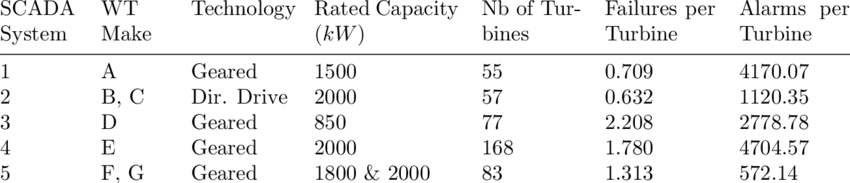
\includegraphics[scale=0.4]{SCADA_table}
	\decoRule
	\caption{Data used for the SCADA Alarms and Failure Analysis \cite{wind_turbine_failures}}
	\label{fig:SCADA_table}
\end{figure}

According to a study on wind turbine accidents \cite{wind_turbine_accidents}, there are 4 main categories of accidents.  These include transportation, construction, operation, and maintenance accidents, which can be caused by either nature, human error, or equipment failure.  According to the study, operation accidents are significantly more common than any other category of failures \cite{wind_turbine_failures}.  Most of the operation accidents (about 80\%) are caused by either equipment failures or nature events.  The detection method outlined in this document would hopefully be able to prevent many of the operation-based accidents, which are a majority of the turbine accidents.

\section{Tower Vibration Research}
Wind turbine tower vibrations are important to the health of turbines and have been studied before.  In one study, a nonlinear state estimation technique \cite{NSET_vibration_modeling} (NSET) is used to attempt to predict wind turbine failures.  This model uses SCADA data to relate different operating parameters to the health of the turbine.  Typically, many variables are used as inputs to determine turbine health and status because vibration alone isn't always sufficient \cite{NSET_vibration_modeling}.  When many variables are used, statistical model become significantly more complex and require large-scale optimization processes which is where machine learning models accel.

Most tower vibration analyses are empirically derived because of the stochastic nature of the wind speed and the amount of variables affecting the turbine.  Data-driven models \cite{data_driven_online_monitoring} are very common in the wind power space, especially with monitoring systems such as SCADA.

\section{Small turbine monitoring system}
As previously discussed, there are a lot of options for large-scale turbine monitoring, but they are expensive and difficult to implement and maintain because many of them need to be directly integrated with the turbine computer to collect the necessary data.  Small-scale turbine systems don't have all of the same requirements as the large-scale systems.  It is valuable to have a lightweight and inexpensive device that can monitor the health of a turbine without requiring direct integration to internal operation parameters.  Ideally, this device should be able to detect impending problems, halt operation, and notify the maintenance operator.

A small-turbine monitoring system would reduce the frequency of maintenance because it would only need to be checked when the system reports possible trouble.  It would also reduce the operation and maintenance cost by stopping all operations when there is a possible problem.  Because this device won't have access to internal operating parameters (such as generator power, internal temperature, rotor speed, wind speed, and wind direction), it will need to monitor the turbine vibrations, which can efficiently be done using accelerometers.  One common turbine problem is a rotor imbalance, caused by either blade damage, loose fasteners, or build-up material on the blades.  If the monitoring device can detect these imbalances, the turbine can be fixed before any additional damage is done.

Additionally, an ideal monitoring device would be wireless and battery-powered.  This means the processor should be very low-power and will need very efficient algorithms and data processing methods when acquiring data and making predictions.  This document will discuss various signal processing methods and their efficiencies, along with analyzing a few machine learning models for rotor imbalance predictions.



